% ! TeX program = lualatex

\documentclass[a0paper,landscape]{tikzposter}

%---------------------------------------------------------------
% Font
%---------------------------------------------------------------
\usepackage[czech,main=english]{babel}
\usepackage[T1]{fontenc}

\usepackage{fontspec}
\setmainfont[
   Path = fonts/,
   BoldFont = Technika-Bold.ttf,
   ItalicFont = Technika-Italic.ttf,
]{Technika-Regular.ttf}
\setsansfont{Technika-Regular.ttf}[Path=fonts/]

\newfontfamily\technikaStencil{TechnikaStencil-Bold.ttf}[Path=fonts/]

%---------------------------------------------------------------
% Packages
%---------------------------------------------------------------
% symbols, fonts
\usepackage{amsmath}
\usepackage{amsfonts}
\usepackage{amsthm}
\usepackage{amssymb}
\usepackage{mathrsfs}

\usepackage{graphicx} % include image
\usepackage{xcolor} % colors
\usepackage{graphicx} % Allows including images

\usepackage{hyperref} % setup links
\usepackage{caption} % \captionof
\usepackage{minted} % Listings
\usepackage{changepage} % \adjustwidth

\usepackage{csquotes} % quoting

\usepackage{titlesec} % format paragraph

\usepackage[style=iso-numeric]{biblatex}
\addbibresource{bib-database.bib}
% \bibliographystyle{ieeetr}

%---------------------------------------------------------------
% Theme
%---------------------------------------------------------------
\usepackage{fittheme}
\tikzposterlatexaffectionproofoff
\usetheme{FITTheme}
\usecolorstyle{FITStyle}

% Links
\hypersetup{
    pdfpagelayout=TwoPageRight,
    colorlinks=false,
    allcolors=decoration,
    pdfborder={0 0 0.1},
    allbordercolors=FITBlue
}

% Minted
\setminted{linenos=false,highlightcolor=SkyBlue}
\usemintedstyle{borland}

\newcommand{\mintoneline}[2]{\mint[linenos=false]{#1}{#2}}

% paragraph
\titleformat{\paragraph}[block]{\normalfont\bfseries}{\theparagraph}{1em}{}
\titlespacing*{\paragraph}{0pt}{0pt}{0em}

%---------------------------------------------------------------
% Title
%---------------------------------------------------------------
\title{Understanding Feedback Pollution in the R Programming Language}
\author{\textbf{Ing. Filip Říha} \hspace{3em}}
\supervisor{Supervisor: doc. Ing. Filip Křikava\, Ph.D.}
\institute{Faculty of Information Technology, Czech Technical University}
\titlegraphic{\centering
\includegraphics[width=0.11\textwidth]{logo/information_technology_negativ.pdf}}

%---------------------------------------------------------------
% Footer
%---------------------------------------------------------------
\footer{
  \centering
  \noindent
  \begin{minipage}{0.5\textwidth-10pt}
      \raggedright
      \textbf{Ř Compiler: \url{https://github.com/reactorlabs/rir}}
  \end{minipage}%
  \begin{minipage}{0.5\textwidth-50pt}
      \raggedleft
      \textbf{IT SPY 2025}
  \end{minipage}%
}

%---------------------------------------------------------------
% Document
%---------------------------------------------------------------
\begin{document}
\maketitle
\centering
\begin{columns}
	%---------------------------------------------------------------
	% Column 1
	%---------------------------------------------------------------
	\column{0.32}

	%---------------------------------------------------------------
	\block{Motivation}
	%---------------------------------------------------------------
	{
		Many modern dynamic languages are executed on a \textit{virtual machine} (VM). To speed up the programs, VMs traditionally include \textit{Just-in-Time} (JIT) compilers, allowing them to improve the performance of frequently executed pieces of programs by compiling them to native code.

    To further enhance performance, during the execution of unoptimized code (in the \textit{interpreter}) VMs record information about the runtime (called \textit{feedback}, stored in a \textit{feedback vector} composed of \textit{slots}), allowing them to predict future behavior. If the feedback information is useful, the compiler speculates on it, leading to a more optimized code if the assumption holds. \\

		Let's take the following JavaScript function:

		\inputminted{js}{listing/example.js}
		\vspace{1em}

		By calling
		\mintoneline{js}{sum(rangeDouble(1, 1e8)) // Peak execution time: 100ms}
		we observe the type \texttt{double}. After a few invocations, a compilation will be triggered, assuming the input is of type \texttt{double}. This allows the JIT to generate optimized native code that approaches C code performance.\\

		If we then call
		\mintoneline{js}{sum(rangeBigInt(1, 1e8)) // Peak execution time: 500ms}
		we update the observed types to both \texttt{double} and \texttt{BigInt}. The assumption on the type is broken, thus a new native version is compiled with weaker assumptions, resulting in less optimized code.\\

		Even if we call again
		\mintoneline{js}{sum(rangeDouble(1, 1e8)) // Peak execution time: 500ms}
		we do not reach the previously observed performance -- this is called \textbf{feedback pollution}.
	}

	%---------------------------------------------------------------
	\block{Goals}
	%---------------------------------------------------------------
	{
		We look at feedback pollution in the context of \textit{R programming language}, a high-level programming language specialized for statistical computing and data visualization.\\

		More concretely, we analyze the pollution in the \textit{Ř Just-in-Time compiler}, developed at CTU Prague and Northeastern University, Boston.
	}

	%---------------------------------------------------------------
	% Column 2
	%---------------------------------------------------------------
	\column{0.36}

	%---------------------------------------------------------------
	\block{Recording Tool}
	%---------------------------------------------------------------
	{
		In order to observe the behavior of Ř, we developed a tool for capturing and recording various events happening in runtime. This resulted in a tool that seamlessly integrates into the compiler, not impacting it at all if not required.  \\

		The result of a recording is illustrated graphically in figure \ref{fig:recorder}. We can see the function invocations, compilations, deoptimizations, and observed types. \\

		\begin{center}
			\begin{adjustwidth}{-3cm}{-3cm}
				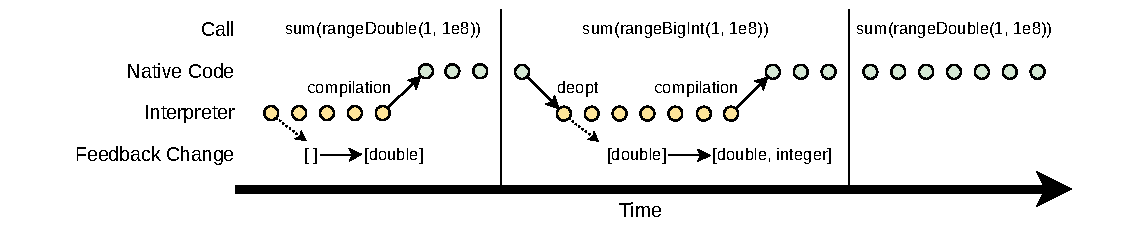
\includegraphics[width=0.36\textwidth]{diagrams/Recording Tool.pdf}
			\end{adjustwidth}
			\captionof{figure}{Graphical illustration of the recording tool result}\label{fig:recorder}
		\end{center}
		\vspace{0.5em}

		\paragraph*{Design Goals}
		\begin{itemize}
			\item{} Capture the behavior of the compiler --- function invocations, compilations, deoptimizations, and feedback updates
			\item{} Minimize the impact on the compiler performance
			\item{} Keep the changes in the compiler code minimal
		\end{itemize}


		\paragraph*{Assessment} The implementation is in less than 1700 lines of code, excluding blank lines and comments.

    Apart from 40 calls to the recording functions, no changes were implemented in the compiler.

		The tool needs to be explicitly enabled in compilation; otherwise, it has no impact on the compiler and its performance.
	}

	%---------------------------------------------------------------
	\block{Analysis of Feedback Pollution}
	%---------------------------------------------------------------
	{
		This was the first usage of the recording tool, published in a 2024 VMIL paper.

		\textit{(Krynski, Sebastián; Štěpánek, Michal; Říha, Filip; Křikava, Filip; Vitek, Jan. Reducing Feedback Pollution. VMIL ’24. DOI: \href{https://doi.org/10.1145/3689490.3690404}{10.1145/3689490.3690404.})}\\

		\paragraph*{Research Question} How does feedback pollution manifest in R?\\

		\paragraph*{Methodology}
		% We define:
		% \begin{itemize}
		% 	\item{} \textit{polluted feedback slot} -- slot whose value at the point of compilation has changed from previous compilation
		% 	\item{} \textit{feedback pollution} -- ratio of the number of modified feedback slots to the total number of feedback slots
		% 	\item{} \textit{polluted compilation} -- compilation, with feedback pollution
		% \end{itemize}
		We define a \textit{polluted feedback slot} as a slot whose value at the point of compilation has changed from previous compilation.

		The experiment was run on Ř benchmarks and one real-life script.

		Data was collected using the recording tool.\\

		\paragraph*{Results} Most functions compiled multiple times have about a quarter of slots polluted. Pollution mostly manifests in polymorphic functions or in functions that heavily use the global state. \\


		% Summary of the results:
		%
		% \begin{tabular}{llll}
		% 	\hline
		% 	                      & Kaggle      & Benchmarks  \\
		% 	\hline
		% 	Lines of code         & 108         & 1268        \\
		% 	Compilations          & 970         & 257         \\
		% 	Polluted compilations & 90 (10.9\%) & 21 (8.2\%)  \\
		% 	Compiled functions    & 315         & 139         \\
		% 	Polluted functions    & 66 (21\%)   & 21 (15.1\%) \\
		% 	\hline
		% \end{tabular}

	}

	%---------------------------------------------------------------
	% Column 3
	%---------------------------------------------------------------
	\column{0.32}

	%---------------------------------------------------------------
	\block{Analysis of Feedback Usage}
	%---------------------------------------------------------------
	{
		After observing that feedback can be polluted, our next step is to understand how the feedback is used in a compilation. The interpreter spends significant time on recording runtime information in hopes that it will make up for it by JIT compiling more optimized code. We want to analyze whether this hypothesis is true and whether there is room for improvement by reducing the amount of information recorded.\\

		These partial results are part of an upcoming publication.\\

		\paragraph*{Research Questions}
		\begin{itemize}
			\item[]\textbf{RQ1:} How much of the recorded information is used?
			\item[]\textbf{RQ2:} Why a slot is not used?
			\item[]\textbf{RQ3:} How does pollution affect the slot usage?\\
		\end{itemize}

		\paragraph*{Methodology} We define:
		\begin{itemize}
			\item{} \textit{non-empty slot} -- has at least one observation
			\item{} \textit{referenced slot} -- it is part of a compiled function
			\item{} \textit{read slot} -- the information is observed during compilation
			\item{} \textit{used slot} -- there is a speculation on this slot
		\end{itemize}

		The experiment was run on a few selected Ř benchmarks and one real-life script.\\

		\paragraph*{Results} The usage of slots on average per compilation:\\

		\begin{centering}
			\begin{adjustwidth}{-1.5cm}{-3cm}
				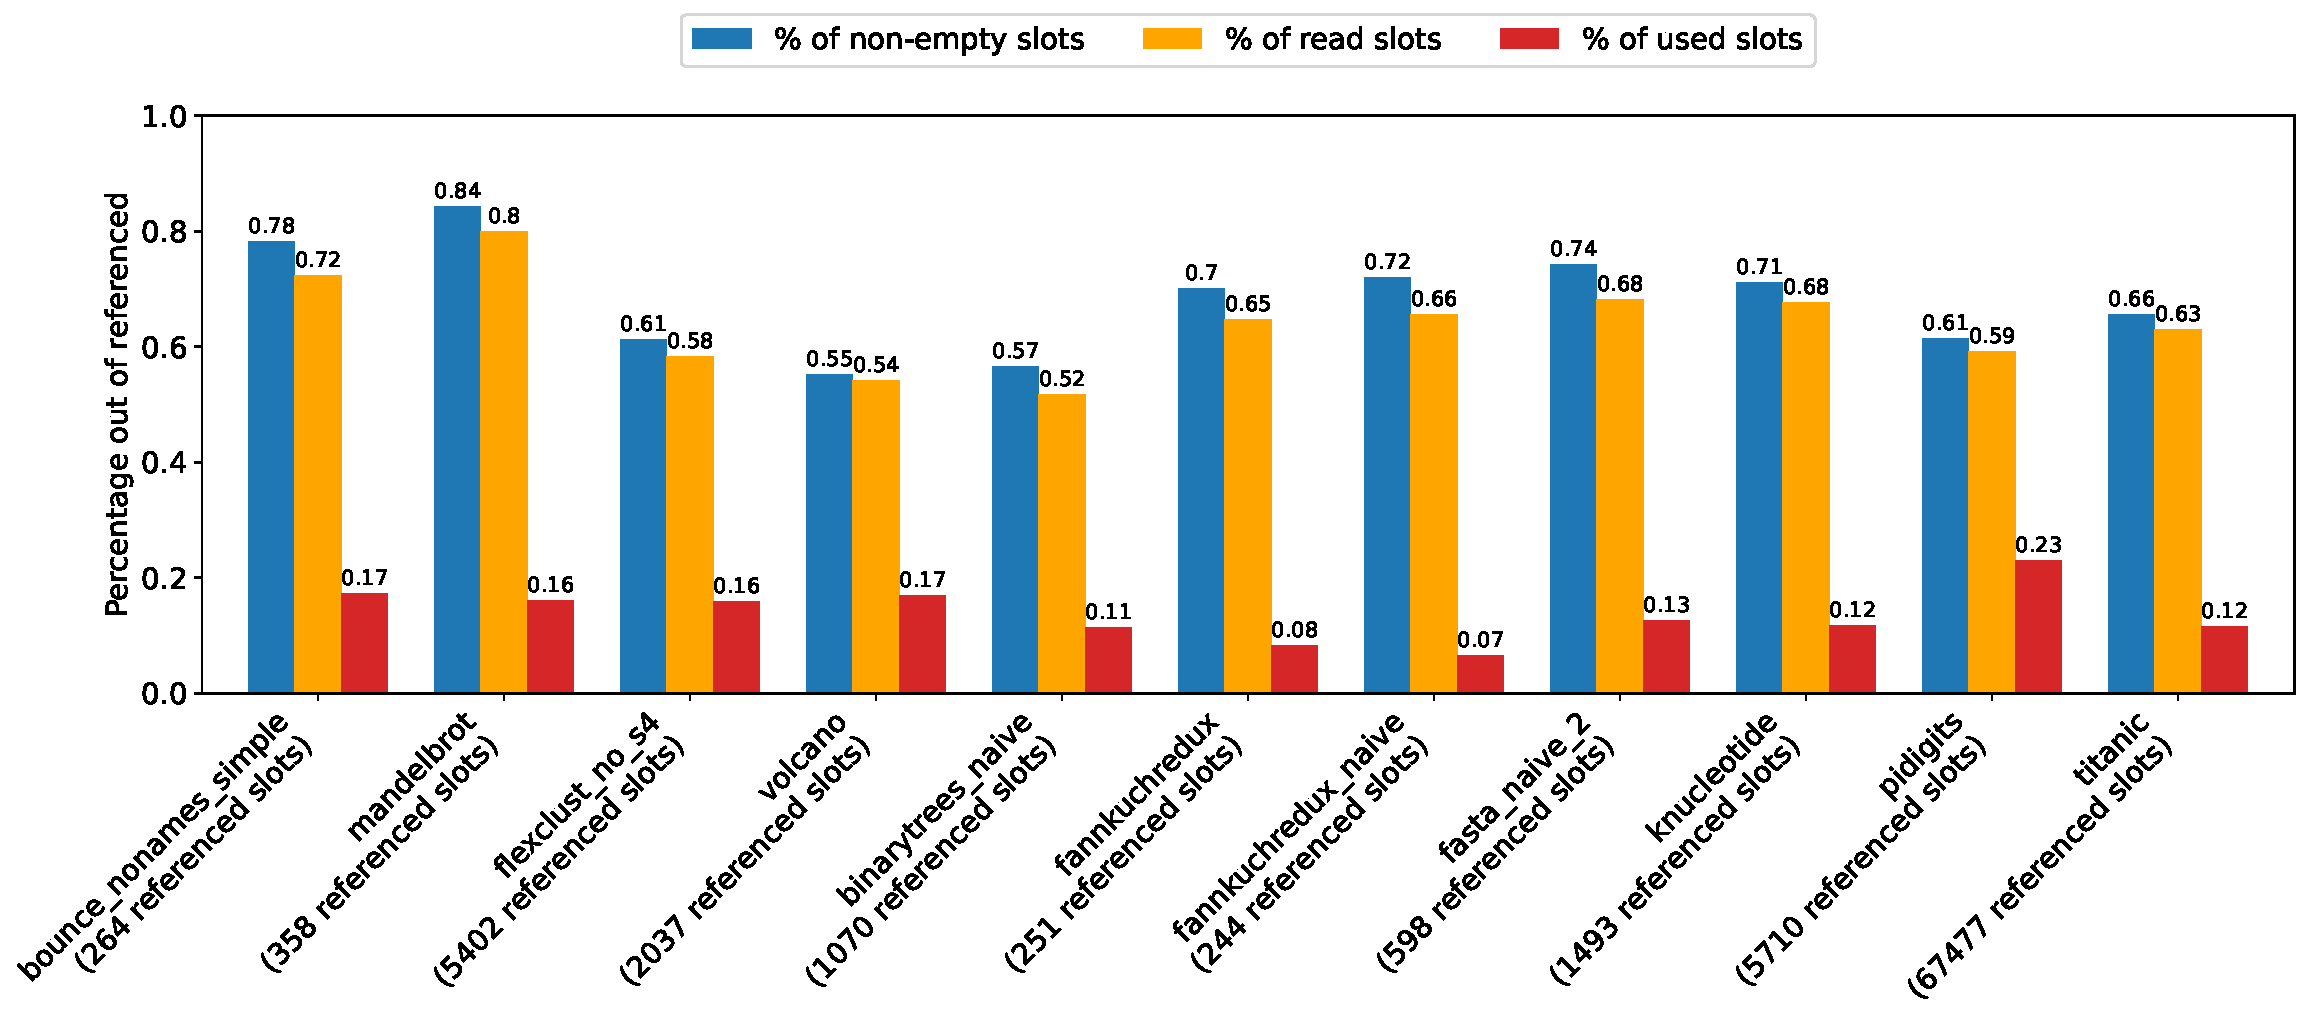
\includegraphics[width=0.31\textwidth]{figures/usage_overall.pdf}
			\end{adjustwidth}
		\end{centering}

		On average, a compilation uses 21\% of non-empty slots. (\textbf{RQ1}) \\

		The main reason for not using a slot is redundancy --- it contains the same information as some other slot. (\textbf{RQ2}) \\

		Pollution of slots does not affect whether a slot is used, but it heavily weakens the assumptions the compiler can make. (\textbf{RQ3}). \\
	}

\end{columns}
% %---------------------------------------------------------------
% \block{}
% %---------------------------------------------------------------
% {
% 	\begin{scriptsize}
% 		\printbibliography[heading=none]
% 	\end{scriptsize}
% }
\end{document}
